\documentclass[12pt]{article}

%packages
%\usepackage{latexsym}
\usepackage{graphicx}
\usepackage{color}
\usepackage{amsmath}
%\usepackage{dsfont}
\usepackage{placeins}
\usepackage{amssymb}
\usepackage{enumerate}
%\usepackage{pstricks,pst-node,pst-tree}

%\usepackage{algpseudocode}
%\usepackage{amsthm}
%\usepackage{hyperref}
%\usepackage{mathrsfs}
%\usepackage{amsfonts}
%\usepackage{bbding}
\usepackage{listings}
\usepackage{appendix}
\usepackage{subfigure}
\usepackage[margin=0.9in]{geometry}
%\geometry{papersize={8.5in,11in},total={6.5in,9in}}
\usepackage{cancel}
%\usepackage{algorithmic, algorithm}
\usepackage{array,colortbl,booktabs}
\usepackage{epstopdf}

\lstset{language = R, numbers = left, backgroundcolor = \color{backgcode}, title = \lstname, breaklines = true, basicstyle = \small, commentstyle = \footnotesize\color{Brown}, stringstyle = \ttfamily, tabsize = 2, fontadjust = true, showspaces = false, showstringspaces = false, texcl = true, numbers = none} %texcl = true, 

%create definition to allow local margin changes
\def\changemargin#1#2{\list{}{\rightmargin#2\leftmargin#1}\item[]}
\let\endchangemargin=\endlist 

%allow equations to span multiple pages
\allowdisplaybreaks

%define colors and color typesetting conveniences
\definecolor{gray}{rgb}{0.8,0.8,0.8}
\definecolor{black}{rgb}{0,0,0}
\definecolor{white}{rgb}{1,1,1}
\definecolor{blue}{rgb}{0,0,1}
\newcommand{\inblue}[1]{\color{blue}#1\color{black}}
\definecolor{backgcode}{rgb}{0.97,0.97,0.8}
\definecolor{Brown}{cmyk}{0,0.81,1,0.60}
\definecolor{OliveGreen}{cmyk}{0.64,0,0.95,0.40}
\definecolor{CadetBlue}{cmyk}{0.62,0.57,0.23,0}

\newcommand{\grayhline}{\arrayrulecolor{gray}\hline\arrayrulecolor{black}}


%define new math operators
\DeclareMathOperator*{\argmax}{arg\,max~}
\DeclareMathOperator*{\argmin}{arg\,min~}
\DeclareMathOperator*{\argsup}{arg\,sup~}
\DeclareMathOperator*{\arginf}{arg\,inf~}
\DeclareMathOperator*{\convolution}{\text{\Huge{$\ast$}}}
\newcommand{\infconv}[2]{\convolution^\infty_{#1 = 1} #2}
%true functions

%%%% GENERAL SHORTCUTS

%shortcuts for pure typesetting conveniences
\newcommand{\bv}[1]{\boldsymbol{#1}}

%shortcuts for compound constants
\newcommand{\BetaDistrConst}{\dfrac{\Gamma(\alpha + \beta)}{\Gamma(\alpha)\Gamma(\beta)}}
\newcommand{\NormDistrConst}{\dfrac{1}{\sqrt{2\pi\sigma^2}}}

%shortcuts for conventional symbols
\newcommand{\tsq}{\tau^2}
\newcommand{\tsqh}{\hat{\tau}^2}
\newcommand{\sigsq}{\sigma^2}
\newcommand{\sigsqmu}{\sigsq_\mu}
\newcommand{\sigsqsq}{\parens{\sigma^2}^2}
\newcommand{\sigsqovern}{\dfrac{\sigsq}{n}}
\newcommand{\tausq}{\tau^2}
\newcommand{\tausqalpha}{\tau^2_\alpha}
\newcommand{\tausqbeta}{\tau^2_\beta}
\newcommand{\tausqsigma}{\tau^2_\sigma}
\newcommand{\betasq}{\beta^2}
\newcommand{\sigsqvec}{\bv{\sigma}^2}
\newcommand{\sigsqhat}{\hat{\sigma}^2}
\newcommand{\sigsqhatmlebayes}{\sigsqhat_{\text{Bayes, MLE}}}
\newcommand{\sigsqhatmle}[1]{\sigsqhat_{#1, \text{MLE}}}
\newcommand{\bSigma}{\bv{\Sigma}}
\newcommand{\bSigmainv}{\bSigma^{-1}}
\newcommand{\thetavec}{\bv{\theta}}
\newcommand{\thetahat}{\hat{\theta}}
\newcommand{\betahat}{\hat{\beta}}
\newcommand{\thetahatmle}{\hat{\theta}_{\mathrm{MLE}}}
\newcommand{\thetavechatmle}{\hat{\thetavec}_{\mathrm{MLE}}}
\newcommand{\muhat}{\hat{\mu}}
\newcommand{\musq}{\mu^2}
\newcommand{\muvec}{\bv{\mu}}
\newcommand{\muhatmle}{\muhat_{\text{MLE}}}
\newcommand{\lambdahat}{\hat{\lambda}}
\newcommand{\lambdahatmle}{\lambdahat_{\text{MLE}}}
\newcommand{\etavec}{\bv{\eta}}
\newcommand{\alphavec}{\bv{\alpha}}
\newcommand{\minimaxdec}{\delta^*_{\mathrm{mm}}}
\newcommand{\ybar}{\bar{y}}
\newcommand{\xbar}{\bar{x}}
\newcommand{\Xbar}{\bar{X}}
\newcommand{\Rbar}{\bar{R}}
\newcommand{\iid}{~{\buildrel iid \over \sim}~}
\newcommand{\inddist}{~{\buildrel ind \over \sim}~}
\newcommand{\approxdist}{~{\buildrel approx \over \sim}~}
\newcommand{\equalsindist}{~{\buildrel d \over =}~}
\newcommand{\equalsquestion}{~{\buildrel ? \over =}~}
\newcommand{\loglik}[1]{\ell\parens{#1}}
\newcommand{\thetahatkminone}{\thetahat^{(k-1)}}
\newcommand{\thetahatkplusone}{\thetahat^{(k+1)}}
\newcommand{\thetahatk}{\thetahat^{(k)}}
\newcommand{\half}{\frac{1}{2}}
\newcommand{\third}{\frac{1}{3}}
\newcommand{\twothirds}{\frac{2}{3}}
\newcommand{\fourth}{\frac{1}{4}}
\newcommand{\fifth}{\frac{1}{5}}
\newcommand{\sixth}{\frac{1}{6}}

%shortcuts for vector and matrix notation
\newcommand{\Ahat}{\hat{A}}
\newcommand{\A}{\bv{A}}
\newcommand{\At}{\A^T}
\newcommand{\Ainv}{\inverse{\A}}
\newcommand{\B}{\bv{B}}
\newcommand{\K}{\bv{K}}
\newcommand{\Kt}{\K^T}
\newcommand{\Kinv}{\inverse{K}}
\newcommand{\Kinvt}{(\Kinv)^T}
\newcommand{\M}{\bv{M}}
\newcommand{\Bt}{\B^T}
\newcommand{\Q}{\bv{Q}}
\newcommand{\Qt}{\Q^T}
\newcommand{\R}{\bv{R}}
\newcommand{\Rt}{\R^T}
\newcommand{\Z}{\bv{Z}}
\newcommand{\X}{\bv{X}}
\newcommand{\Xsub}{\X_{\text{(sub)}}}
\newcommand{\Xsubadj}{\X_{\text{(sub,adj)}}}
\newcommand{\I}{\bv{I}}
\newcommand{\J}{\bv{J}}
\newcommand{\Y}{\bv{Y}}
\newcommand{\V}{\bv{V}}
\newcommand{\Vinv}{\V^{-1}}
\newcommand{\bzero}{\bv{0}}
\newcommand{\sigsqI}{\sigsq\I}
\renewcommand{\P}{\bv{P}}
\newcommand{\Psub}{\P_{\text{(sub)}}}
\newcommand{\Pt}{\P^T}
\newcommand{\Pii}{P_{ii}}
\newcommand{\Pij}{P_{ij}}
\newcommand{\IminP}{(\I-\P)}
\newcommand{\Xt}{\bv{X}^T}
\newcommand{\XtX}{\Xt\X}
\newcommand{\XtXinv}{\parens{\Xt\X}^{-1}}
\newcommand{\XtXinvXt}{\XtXinv\Xt}
\newcommand{\XXtXinvXt}{\X\XtXinvXt}
\newcommand{\x}{\bv{x}}
\newcommand{\onevec}{\bv{1}}
\newcommand{\onevecp}{\bv{1}_p}
\newcommand{\onevecpt}{\onevecp^T}
\newcommand{\oneton}{1, \ldots, n}
\newcommand{\yoneton}{y_1, \ldots, y_n}
\newcommand{\yonetonorder}{y_{(1)}, \ldots, y_{(n)}}
\newcommand{\Yoneton}{Y_1, \ldots, Y_n}
\newcommand{\iinoneton}{i \in \braces{\oneton}}
\newcommand{\onetom}{1, \ldots, m}
\newcommand{\jinonetom}{j \in \braces{\onetom}}
\newcommand{\xoneton}{x_1, \ldots, x_n}
\newcommand{\Xoneton}{X_1, \ldots, X_n}
\newcommand{\Roneton}{R_1, \ldots, R_n}
\newcommand{\Rlonetonl}{R_{\ell_1}, \ldots, R_{\ell_{n_\ell}}}
\newcommand{\RLlonetonlL}{R_{\ell_{L,1}}, \ldots, R_{\ell_{L, n_{\ell,L}}}}
\newcommand{\RRlonetonlR}{R_{\ell_{R,1}}, \ldots, R_{R,\ell_{n_{\ell,R}}}}
\newcommand{\xt}{\x^T}
\newcommand{\y}{\bv{y}}
\newcommand{\yt}{\y^T}
\renewcommand{\c}{\bv{c}}
\newcommand{\ct}{\c^T}
\newcommand{\tstar}{\bv{t}^*}
\renewcommand{\u}{\bv{u}}
\renewcommand{\v}{\bv{v}}
\renewcommand{\a}{\bv{a}}
\newcommand{\s}{\bv{s}}
\newcommand{\yadj}{\y_{\text{(adj)}}}
\newcommand{\xjadj}{\x_{j\text{(adj)}}}
\newcommand{\xjadjM}{\x_{j \perp M}}
\newcommand{\yhat}{\hat{\y}}
\newcommand{\yhatsub}{\yhat_{\text{(sub)}}}
\newcommand{\yhatstar}{\yhat^*}
\newcommand{\yhatstarnew}{\yhatstar_{\text{new}}}
\newcommand{\z}{\bv{z}}
\newcommand{\zt}{\z^T}
\newcommand{\bb}{\bv{b}}
\newcommand{\bbt}{\bb^T}
\newcommand{\bbeta}{\bv{\beta}}
\newcommand{\bbetat}{\bbeta^T}
\newcommand{\beps}{\bv{\epsilon}}
\newcommand{\bepst}{\beps^T}
\newcommand{\e}{\bv{e}}
\newcommand{\Mofy}{\M(\y)}
\newcommand{\KofAlpha}{K(\alpha)}
\newcommand{\ellset}{\mathcal{L}}
\newcommand{\oneminalph}{1-\alpha}
\newcommand{\SSE}{\text{SSE}}
\newcommand{\SSEsub}{\text{SSE}_{\text{(sub)}}}
\newcommand{\MSE}{\text{MSE}}
\newcommand{\RMSE}{\text{RMSE}}
\newcommand{\SSR}{\text{SSR}}
\newcommand{\SST}{\text{SST}}
\newcommand{\JSest}{\delta_{\text{JS}}(\x)}
\newcommand{\Bayesest}{\delta_{\text{Bayes}}(\x)}
\newcommand{\EmpBayesest}{\delta_{\text{EmpBayes}}(\x)}
\newcommand{\BLUPest}{\delta_{\text{BLUP}}}
\newcommand{\MLEest}[1]{\hat{#1}_{\text{MLE}}}
\newcommand{\errordist}{\mathcal{E}}
\newcommand{\berrordist}{\bv{\errordist}}
\newcommand{\error}{\varepsilon}



%shortcuts for Linear Algebra stuff (i.e. vectors and matrices)
\newcommand{\twovec}[2]{\bracks{\begin{array}{c} #1 \\ #2 \end{array}}}
\newcommand{\threevec}[3]{\bracks{\begin{array}{c} #1 \\ #2 \\ #3 \end{array}}}
\newcommand{\fivevec}[5]{\bracks{\begin{array}{c} #1 \\ #2 \\ #3 \\ #4 \\ #5 \end{array}}}
\newcommand{\twobytwomat}[4]{\bracks{\begin{array}{cc} #1 & #2 \\ #3 & #4 \end{array}}}
\newcommand{\threebytwomat}[6]{\bracks{\begin{array}{cc} #1 & #2 \\ #3 & #4 \\ #5 & #6 \end{array}}}

%shortcuts for conventional compound symbols
\newcommand{\thetainthetas}{\theta \in \Theta}
\newcommand{\reals}{\mathbb{R}}
\newcommand{\complexes}{\mathbb{C}}
\newcommand{\rationals}{\mathbb{Q}}
\newcommand{\integers}{\mathbb{Z}}
\newcommand{\naturals}{\mathbb{N}}
\newcommand{\forallninN}{~~\forall n \in \naturals}
\newcommand{\forallxinN}[1]{~~\forall #1 \in \reals}
\newcommand{\matrixdims}[2]{\in \reals^{\,#1 \times #2}}
\newcommand{\inRn}[1]{\in \reals^{\,#1}}
\newcommand{\mathimplies}{\quad\Rightarrow\quad}
\newcommand{\mathlogicequiv}{\quad\Leftrightarrow\quad}
\newcommand{\eqncomment}[1]{\quad \text{(#1)}}
\newcommand{\limitn}{\lim_{n \rightarrow \infty}}
\newcommand{\limitN}{\lim_{N \rightarrow \infty}}
\newcommand{\limitd}{\lim_{d \rightarrow \infty}}
\newcommand{\limitt}{\lim_{t \rightarrow \infty}}
\newcommand{\limitsupn}{\limsup_{n \rightarrow \infty}~}
\newcommand{\limitinfn}{\liminf_{n \rightarrow \infty}~}
\newcommand{\limitk}{\lim_{k \rightarrow \infty}}
\newcommand{\limsupn}{\limsup_{n \rightarrow \infty}}
\newcommand{\limsupk}{\limsup_{k \rightarrow \infty}}
\newcommand{\floor}[1]{\left\lfloor #1 \right\rfloor}
\newcommand{\ceil}[1]{\left\lceil #1 \right\rceil}


%shortcuts for environments
\newcommand{\beqn}{\vspace{-0.25cm}\begin{eqnarray*}}
\newcommand{\eeqn}{\end{eqnarray*}}
\newcommand{\bneqn}{\vspace{-0.25cm}\begin{eqnarray}}
\newcommand{\eneqn}{\end{eqnarray}}

%shortcuts for mini environments
\newcommand{\parens}[1]{\left(#1\right)}
\newcommand{\squared}[1]{\parens{#1}^2}
\newcommand{\squaredfrac}[2]{\squared{\frac{#1}{#2}}}
\newcommand{\tothepow}[2]{\parens{#1}^{#2}}
\newcommand{\prob}[1]{\mathbb{P}\parens{#1}}
\newcommand{\cprob}[2]{\prob{#1 \, \big| \, #2}}
\newcommand{\littleo}[1]{o\parens{#1}}
\newcommand{\bigo}[1]{O\parens{#1}}
\newcommand{\Lp}[1]{\mathbb{L}^{#1}}
\renewcommand{\arcsin}[1]{\text{arcsin}\parens{#1}}
\newcommand{\prodonen}[2]{\prod_{#1=1}^n #2}
\newcommand{\mysum}[4]{\sum_{#1=#2}^{#3} #4}
\newcommand{\sumonen}[2]{\sum_{#1=1}^n #2}
\newcommand{\infsum}[2]{\sum_{#1=1}^\infty #2}
\newcommand{\infprod}[2]{\prod_{#1=1}^\infty #2}
\newcommand{\infunion}[2]{\bigcup_{#1=1}^\infty #2}
\newcommand{\infinter}[2]{\bigcap_{#1=1}^\infty #2}
\newcommand{\infintegral}[2]{\int^\infty_{-\infty} #2 ~\text{d}#1}
\newcommand{\supthetas}[1]{\sup_{\thetainthetas}\braces{#1}}
\newcommand{\bracks}[1]{\left[#1\right]}
\newcommand{\braces}[1]{\left\{#1\right\}}
\newcommand{\set}[1]{\left\{#1\right\}}
\newcommand{\abss}[1]{\left|#1\right|}
\newcommand{\norm}[1]{\left|\left|#1\right|\right|}
\newcommand{\normsq}[1]{\norm{#1}^2}
\newcommand{\inverse}[1]{\parens{#1}^{-1}}
\newcommand{\transpose}[1]{\parens{#1}^{\top}}
\newcommand{\rowof}[2]{\parens{#1}_{#2\cdot}}

%shortcuts for functionals
\newcommand{\realcomp}[1]{\text{Re}\bracks{#1}}
\newcommand{\imagcomp}[1]{\text{Im}\bracks{#1}}
\newcommand{\range}[1]{\text{range}\bracks{#1}}
\newcommand{\colsp}[1]{\text{colsp}\bracks{#1}}
\newcommand{\rowsp}[1]{\text{rowsp}\bracks{#1}}
\newcommand{\tr}[1]{\text{tr}\bracks{#1}}
\newcommand{\rank}[1]{\text{rank}\bracks{#1}}
\newcommand{\proj}[2]{\text{Proj}_{#1}\bracks{#2}}
\newcommand{\projcolspX}[1]{\text{Proj}_{\colsp{\X}}\bracks{#1}}
\newcommand{\median}[1]{\text{median}\bracks{#1}}
\newcommand{\mean}[1]{\text{mean}\bracks{#1}}
\newcommand{\dime}[1]{\text{dim}\bracks{#1}}
\renewcommand{\det}[1]{\text{det}\bracks{#1}}
\newcommand{\diag}[1]{\text{diag}\bracks{#1}}
\newcommand{\expe}[1]{\mathbb{E}\bracks{#1}}
\newcommand{\expeabs}[1]{\expe{\abss{#1}}}
\newcommand{\expesub}[2]{\mathbb{E}_{#1}\bracks{#2}}
\newcommand{\indic}[1]{\mathbb{I}_{#1}}
\newcommand{\var}[1]{\mathbb{V}\text{ar}\bracks{#1}}
\newcommand{\cov}[2]{\mathbb{C}\,\text{ov}\bracks{#1, #2}}
\newcommand{\corr}[2]{\text{Corr}\bracks{#1, #2}}
\newcommand{\se}[1]{\text{SE}\bracks{#1}}
\newcommand{\seest}[1]{\hat{\text{SE}}\bracks{#1}}
\newcommand{\bias}[1]{\text{Bias}\bracks{#1}}
\newcommand{\partialop}[2]{\dfrac{\partial}{\partial #1}\bracks{#2}}
\newcommand{\secpartialop}[2]{\dfrac{\partial^2}{\partial #1^2}\bracks{#2}}
\newcommand{\mixpartialop}[3]{\dfrac{\partial^2}{\partial #1 \partial #2}\bracks{#3}}

%shortcuts for functions
\renewcommand{\exp}[1]{\mathrm{exp}\parens{#1}}
\renewcommand{\cos}[1]{\text{cos}\parens{#1}}
\renewcommand{\sin}[1]{\text{sin}\parens{#1}}
\renewcommand{\cot}[1]{\text{cot}\parens{#1}}
\newcommand{\cotsq}[1]{\text{cot}^2\parens{#1}}
\newcommand{\sign}[1]{\text{sign}\parens{#1}}
\newcommand{\are}[1]{\mathrm{ARE}\parens{#1}}
\newcommand{\natlog}[1]{\ln\parens{#1}}
\newcommand{\logit}[1]{\text{logit}\parens{#1}}
\newcommand{\oneover}[1]{\frac{1}{#1}}
\newcommand{\doneover}[1]{\dfrac{1}{#1}}
\newcommand{\overtwo}[1]{\frac{#1}{2}}
\newcommand{\overn}[1]{\frac{#1}{n}}
\newcommand{\oneoversqrt}[1]{\oneover{\sqrt{#1}}}
\newcommand{\doneoversqrt}[1]{\doneover{\sqrt{#1}}}
\newcommand{\sqd}[1]{\parens{#1}^2}
\newcommand{\loss}[1]{\ell\parens{\theta, #1}}
\newcommand{\losstwo}[2]{\ell\parens{#1, #2}}
\newcommand{\cf}{\phi(t)}

%English language specific shortcuts
\newcommand{\ie}{\textit{i.e.} }
\newcommand{\AKA}{\textit{AKA} }
\renewcommand{\iff}{\textit{iff}}
\newcommand{\eg}{\textit{e.g.} }
\newcommand{\st}{\textit{s.t.} }
\newcommand{\wrt}{\textit{w.r.t.} }
\newcommand{\mathst}{~~\text{\st}~~}
\newcommand{\mathand}{~~\text{and}~~}
\newcommand{\ala}{\textit{a la} }
\newcommand{\ppp}{posterior predictive p-value}
\newcommand{\dd}{dataset-to-dataset}

%shortcuts for distribution titles
\newcommand{\logistic}[2]{\mathrm{Logistic}\parens{#1,\,#2}}
\newcommand{\bernoulli}[1]{\mathrm{Bernoulli}\parens{#1}}
\newcommand{\betanot}[2]{\mathrm{Beta}\parens{#1,\,#2}}
\newcommand{\multbetanot}[3]{\mathrm{Beta}_{#1}\parens{#2,\,#3}}
\newcommand{\stdbetanot}{\betanot{\alpha}{\beta}}
\newcommand{\multnormnot}[3]{\mathcal{N}_{#1}\parens{#2,\,#3}}
\newcommand{\wishart}[3]{\mathcal{W}_{#1}\parens{#2,\,#3}}
\newcommand{\normnot}[2]{\mathcal{N}\parens{#1,\,#2}}
\newcommand{\classicnormnot}{\normnot{\mu}{\sigsq}}
\newcommand{\stdnormnot}{\normnot{0}{1}}
\newcommand{\uniform}[2]{\mathrm{U}\parens{#1,\,#2}}
\newcommand{\stduniform}{\uniform{0}{1}}
\newcommand{\exponential}[1]{\mathrm{Exp}\parens{#1}}
\newcommand{\gammadist}[2]{\mathrm{Gamma}\parens{#1, #2}}
\newcommand{\poisson}[1]{\mathrm{Poisson}\parens{#1}}
\newcommand{\binomial}[2]{\mathrm{Binomial}\parens{#1,\,#2}}
\newcommand{\rayleigh}[1]{\mathrm{Rayleigh}\parens{#1}}
\newcommand{\multinomial}[2]{\mathrm{Multinomial}\parens{#1,\,#2}}
\newcommand{\gammanot}[2]{\mathrm{Gamma}\parens{#1,\,#2}}
\newcommand{\cauchynot}[2]{\text{Cauchy}\parens{#1,\,#2}}
\newcommand{\invchisqnot}[1]{\text{Inv}\chisq{#1}}
\newcommand{\invscaledchisqnot}[2]{\text{ScaledInv}\ncchisq{#1}{#2}}
\newcommand{\invgammanot}[2]{\text{InvGamma}\parens{#1,\,#2}}
\newcommand{\chisq}[1]{\chi^2_{#1}}
\newcommand{\ncchisq}[2]{\chi^2_{#1}\parens{#2}}
\newcommand{\ncF}[3]{F_{#1,#2}\parens{#3}}

%shortcuts for PDF's of common distributions
\newcommand{\logisticpdf}[3]{\oneover{#3}\dfrac{\exp{-\dfrac{#1 - #2}{#3}}}{\parens{1+\exp{-\dfrac{#1 - #2}{#3}}}^2}}
\newcommand{\betapdf}[3]{\dfrac{\Gamma(#2 + #3)}{\Gamma(#2)\Gamma(#3)}#1^{#2-1} (1-#1)^{#3-1}}
\newcommand{\normpdf}[3]{\frac{1}{\sqrt{2\pi#3}}\exp{-\frac{1}{2#3}(#1 - #2)^2}}
\newcommand{\mnormpdf}[2]{\oneover{(2\pi)^{#1/2}|\Sigma|^{1/2}}\exp{-\half (x-#2)^T \Siginv (x-#2)}}
\newcommand{\normpdfvarone}[2]{\dfrac{1}{\sqrt{2\pi}}e^{-\half(#1 - #2)^2}}
\newcommand{\chisqpdf}[2]{\dfrac{1}{2^{#2/2}\Gamma(#2/2)}\; {#1}^{#2/2-1} e^{-#1/2}}
\newcommand{\invchisqpdf}[2]{\dfrac{2^{-\overtwo{#1}}}{\Gamma(#2/2)}\,{#1}^{-\overtwo{#2}-1}  e^{-\oneover{2 #1}}}
\newcommand{\exponentialpdf}[2]{#2\exp{-#2#1}}
\newcommand{\poissonpdf}[2]{\dfrac{e^{-#1} #1^{#2}}{#2!}}
\newcommand{\binomialpdf}[3]{\binom{#2}{#1}#3^{#1}(1-#3)^{#2-#1}}
\newcommand{\rayleighpdf}[2]{\dfrac{#1}{#2^2}\exp{-\dfrac{#1^2}{2 #2^2}}}
\newcommand{\gammapdf}[3]{\dfrac{#3^#2}{\Gamma\parens{#2}}#1^{#2-1}\exp{-#3 #1}}
\newcommand{\cauchypdf}[3]{\oneover{\pi} \dfrac{#3}{\parens{#1-#2}^2 + #3^2}}
\newcommand{\Gammaf}[1]{\Gamma\parens{#1}}

%shortcuts for miscellaneous typesetting conveniences
\newcommand{\notesref}[1]{\marginpar{\color{gray}\tt #1\color{black}}}

%%%% DOMAIN-SPECIFIC SHORTCUTS

%Real analysis related shortcuts
\newcommand{\zeroonecl}{\bracks{0,1}}
\newcommand{\forallepsgrzero}{\forall \epsilon > 0~~}
\newcommand{\lessthaneps}{< \epsilon}
\newcommand{\fraccomp}[1]{\text{frac}\bracks{#1}}

%Bayesian related shortcuts
\newcommand{\yrep}{y^{\text{rep}}}
\newcommand{\yrepisq}{(\yrep_i)^2}
\newcommand{\yrepvec}{\bv{y}^{\text{rep}}}


%Probability shortcuts
\newcommand{\SigField}{\mathcal{F}}
\newcommand{\ProbMap}{\mathcal{P}}
\newcommand{\probtrinity}{\parens{\Omega, \SigField, \ProbMap}}
\newcommand{\convp}{~{\buildrel p \over \rightarrow}~}
\newcommand{\convLp}[1]{~{\buildrel \Lp{#1} \over \rightarrow}~}
\newcommand{\nconvp}{~{\buildrel p \over \nrightarrow}~}
\newcommand{\convae}{~{\buildrel a.e. \over \longrightarrow}~}
\newcommand{\convau}{~{\buildrel a.u. \over \longrightarrow}~}
\newcommand{\nconvau}{~{\buildrel a.u. \over \nrightarrow}~}
\newcommand{\nconvae}{~{\buildrel a.e. \over \nrightarrow}~}
\newcommand{\convd}{~{\buildrel \mathcal{D} \over \rightarrow}~}
\newcommand{\nconvd}{~{\buildrel \mathcal{D} \over \nrightarrow}~}
\newcommand{\withprob}{~~\text{w.p.}~~}
\newcommand{\io}{~~\text{i.o.}}

\newcommand{\Acl}{\bar{A}}
\newcommand{\ENcl}{\bar{E}_N}
\newcommand{\diam}[1]{\text{diam}\parens{#1}}

\newcommand{\taua}{\tau_a}

\newcommand{\myint}[4]{\int_{#2}^{#3} #4 \,\text{d}#1}
\newcommand{\laplacet}[1]{\mathscr{L}\bracks{#1}}
\newcommand{\laplaceinvt}[1]{\mathscr{L}^{-1}\bracks{#1}}
\renewcommand{\min}[1]{\text{min}\braces{#1}}

\newcommand{\Vbar}[1]{\bar{V}\parens{#1}}
\newcommand{\expnegrtau}{\exp{-r\tau}}

\newcommand{\Yij}{Y_{ij}}

\newcommand{\pval}{p_{\text{val}}}

\newcommand{\Hint}{H_{\text{internals}}}
\newcommand{\Hleaves}{H_{\text{leaves}}}

\newcommand{\nadj}{n_{p.\text{adj}}}
\newcommand{\nadjstar}{n_{\text{adj}^*}}
\newcommand{\nrep}{n_{\text{repeat}}}
\newcommand{\nrepstar}{n_{\text{repeat}^*}}

%change step stuff
\newcommand{\etastar}{\eta_*}
\newcommand{\etaone}{\eta_1}
\newcommand{\etatwo}{\eta_2}
\newcommand{\etaonestar}{\eta_{1^*}}
\newcommand{\etatwostar}{\eta_{2^*}}

\newcommand{\none}{n_{1}}
\newcommand{\ntwo}{n_{2}}
\newcommand{\Rones}{R_{1,1}, \ldots, R_{1, \none}}
\newcommand{\Rtwos}{R_{2,1}, \ldots, R_{2, \ntwo}}

\newcommand{\nonestar}{n_{1^*}}
\newcommand{\ntwostar}{n_{2^*}}
\newcommand{\Ronestars}{R_{1^*,1}, \ldots, R_{1^*, \nonestar}}
\newcommand{\Rtwostars}{R_{2^*,1}, \ldots, R_{2^*, \ntwostar}}

\newcommand{\Ronebar}{\bar{R}_1}
\newcommand{\Rtwobar}{\bar{R}_2}
\newcommand{\Ronebarstar}{\bar{R}_{1^*}}
\newcommand{\Rtwobarstar}{\bar{R}_{2^*}}


\title{Heteroskedastic BART Augmentation}

\date{}

\newcommand{\treet}[1]{\text{\PHplaneTree}_{#1}}

\begin{document}
\maketitle

\section*{Introduction}

We want to extend the BART model so that each observation now can have its own variance (but each observation is still independent). The model becomes:

\beqn
Y = \sum_{t=1}^m \treet{t}\parens{X_1, \ldots, X_p} + \berrordist, \quad \berrordist \sim \multnormnot{n}{\bv{0}}{\underbrace{\threebythreemat{\sigsq_1}{}{}{}{\ddots}{}{}{}{\sigsq_k}}_{\D}}
\eeqn


We take vanilla BART and now condition on the variances and then we augment the last step of the Gibbs sampler to now do $n$ samples --- one for $\sigsq_1$, one for $\sigsq_2$, $\ldots$, and one for $\sigsq_n$. Remember that $E$ is the $n$-vector of residuals, $Y$ minus the best guess inside the trees:

\beqn
\treet{1} &~|~& R_1, \sigsq_1, \ldots, \sigsq_n \\
M_1 &~|~& \treet{1}, R_1, \sigsq_1, \ldots, \sigsq_n \\
\vdots && \\
\treet{m} &~|~& R_m, \sigsq_1, \ldots, \sigsq_n \\
M_m &~|~& \treet{m}, R_m, \sigsq_1, \ldots, \sigsq_n \\
\sigsq_1 &~|~& E \\
\vdots && \\
\sigsq_n &~|~& E \\
\eeqn

Thus, there are many pieces in the BART model that will now have to be altered. Each subsection below is devoted to each piece.

\pagebreak
\subsection*{Prior on the variance}

We present two possible designs below for the prior on the $\sigsq$'s:

\begin{itemize}
\item  We keep the same prior as before, now it's on each of the observation's variances:

\beqn
\sigsq_1, \ldots, \sigsq_n \iid \invgammanot{\overtwo{\nu}}{\overtwo{\nu\lambda}}
\eeqn

We may have to rethink the above, but it seems like a good start. Once again we pick $\nu = 3$ and we pick $\lambda$ so that 90\% of the prior's density is below $s^2$, our estimate from the data which is either just the sample variance, or the RMSE squared from a linear model. 

\item We also can have individual priors:

\beqn
\sigsq_1 &\sim& \invgammanot{\overtwo{\nu}}{\overtwo{\nu\lambda_1}} \\
\vdots && \\
\sigsq_n &\sim& \invgammanot{\overtwo{\nu}}{\overtwo{\nu\lambda_n}} \\
\eeqn

where $\lambda_i$ is picked based on the weighted least squares residual for each observation.

\end{itemize}

\subsection*{Changes in Gibbs Sampler for $M$}

The other step that has to change is sampling the leaf $\mu$'s. Remember that $M_t ~|~ \treet{1}, R_1, \sigsq_1, \ldots, \sigsq_n$ is actually the sampling for all leaves where each leaf is considered independent:

\beqn
\mu_{t1} &~|~&  \treet{t}, R_{t_1}, \sigsq_1, \ldots, \sigsq_n \\
\vdots && \\
\mu_{tb_t} &~|~&  \treet{t}, R_{t_{b_t}}, \sigsq_1, \ldots, \sigsq_n \\
\eeqn

The subscripts on the $R$ term indicates we only consider the data that falls into the leaf. So remember that the prior on the leaf value was normal, and the likelihood was assumed normal as well. The only thing that changes is we now have a different variance estimate for each observation. 

We derive the correct posterior distribution below. We drop the subscripts just for convenience since it will be the same for each of the above and denote $k$ as the number of data records that fell into this leaf. $\braces{\sigsq_1, \ldots, \sigsq_k} \subset \braces{\sigsq_1, \ldots, \sigsq_n}$ for the data in this leaf as well:

\beqn
\cprob{\mu}{R, \sigsq_1, \ldots, \sigsq_k} &\propto& \cprob{R}{\mu, \sigsq_1, \ldots, \sigsq_n} \cprob{\mu}{\sigsq_1, \ldots, \sigsq_k} \\
&=& \multnormnot{k}{\mu\onevec}{\D} \normnot{0}{\sigsq_\mu} \\
&\vdots& \\
&=& \normnot{\frac{\dfrac{k^2 \Rbar}{\sum_{i=1}^k \sigsq_i}}{\doneover{\sigsq_\mu} + \dfrac{k^2}{\sum_{i=1}^k \sigsq_i}}}{\oneover{\doneover{\sigsq_\mu} + \dfrac{k^2}{\sum_{i=1}^k \sigsq_i}}}
\eeqn

\subsection*{Changes in Gibbs Sampler for $\sigsq_i$}

In vanilla BART, the posterior of $\sigsq$ was:

\beqn
\sigsq ~|~ e_1, \ldots, e_n \sim \invgammanot{\overtwo{\nu + n}}{\overtwo{\lambda\nu + \sum_{i=1}^n e_i^2}} 
\eeqn

Now, we have to sample each $\sigsq_1, \ldots, \sigsq_n$ from their individual posteriors. The analagous expression is that the SSE is based on only one residual:

\beqn
\sigsq_i ~|~ e_i \sim \invgammanot{\overtwo{\nu + 1}}{\overtwo{\lambda\nu + e_i^2}}
\eeqn


\subsection*{Changes in Likelihood for $R$}

In vanilla BART, we had:

\beqn
&& \frac{\cprob{\R}{T^*, \sigsq}}{\cprob{\R}{T, \sigsq}} \\
&=& \frac{\myint{\mu}{\reals}{}{\cprob{\RLlonetonlL}{\mu, \sigsq}\prob{\mu}} ~~ \myint{\mu}{\reals}{}{\cprob{\RRlonetonlR}{\mu, \sigsq}\prob{\mu}}}{\myint{\mu}{\reals}{}{\cprob{\Rlonetonl}{\mu, \sigsq}\prob{\mu}}}  \\
&\vdots& \\
&=& \sqrt{\frac{\sigsq \parens{\sigsq + n_\ell \sigsqmu}}{\parens{\sigsq + n_{\ell_L} \sigsqmu}\parens{\sigsq + n_{\ell_R} \sigsqmu}}}~\exp{\frac{\sigsq_\mu}{2\sigsq} \parens{\frac{\squared{\sum_{i=1}^{n_{\ell_L}} R_{\ell_L, i}}}{\sigsq + n_{\ell_L}\sigsq_\mu} + \frac{\squared{\sum_{i=1}^{n_{\ell_R}} R_{\ell_R, i}}}{\sigsq + n_{\ell_R}\sigsq_\mu} - \frac{\squared{\sum_{i=1}^{n_{\ell}} R_{\ell, i}}}{\sigsq + n_\ell \sigsq_\mu}}} \\
\eeqn

We cannot use this expression as before since $\sigsq$ is no longer shared across all observations. Instead we have to use:

\small
\beqn
&& \frac{\cprob{\R}{T^*, \sigsq_1, \ldots, \sigsq_n}}{\cprob{\R}{T, \sigsq_1, \ldots, \sigsq_n}} \\
&=& \frac{\myint{\mu}{\reals}{}{\cprob{\RLlonetonlL}{\mu, \sigsq_1, \ldots, \sigsq_n}\prob{\mu}} ~~ \myint{\mu}{\reals}{}{\cprob{\RRlonetonlR}{\mu, \sigsq_1, \ldots, \sigsq_n}\prob{\mu}}}{\myint{\mu}{\reals}{}{\cprob{\Rlonetonl}{\mu, \sigsq_1, \ldots, \sigsq_n}\prob{\mu}}} 
\eeqn
\normalsize

Thus, we have to figure out the following below. I'm going to drop the subscripts for convenience:

\beqn
&& \myint{\mu}{\reals}{}{\cprob{\R}{\mu, \sigsq_1, \ldots, \sigsq_n}\prob{\mu}}  \\
&=& \myint{\mu}{\reals}{}{\oneover{\tothepow{2\pi}{\overtwo{n}} \abss{\D}^{-\half}}\exp{-\half\transpose{\R - \mu\onevec} \D^{-1} (\R - \mu\onevec)} ~\oneoversqrt{2\pi\sigsq_\mu} \exp{-\oneover{2\sigsq_\mu} \musq}}~ \\
&=& \myint{\mu}{\reals}{}{\parens{\prod_{i=1}^{n} \oneoversqrt{2\pi\sigsq_i} \exp{-\oneover{2\sigsq_i} \squared{R_i - \mu}}} ~\oneoversqrt{2\pi\sigsq_\mu} \exp{-\oneover{2\sigsq_\mu} \musq}}~ \\
&=& \oneover{\tothepow{2\pi}{\overtwo{n} + 1}\sqrt{\sigsqmu \prod_{i=1}^{n} \sigsq_i}}\myint{\mu}{\reals}{}{\exp{-\half \parens{\musq + \sumonen{i}{\squared{R_i - \mu}}} }}\\
&=& \oneover{\tothepow{2\pi}{\overtwo{n} + 1}\sqrt{\sigsqmu \prod_{i=1}^{n} \sigsq_i}}\myint{\mu}{\reals}{}{\exp{-\half \parens{\frac{\musq}{\sigsq_\mu} + \sumonen{i}{\frac{R_i^2}{\sigsq_i} - \frac{2\mu R_i}{\sigsq_i} + \frac{\musq}{\sigsq_i}}} }}\\
&=& \oneover{\tothepow{2\pi}{\overtwo{n} + 1}\sqrt{\sigsqmu \prod_{i=1}^{n} \sigsq_i}}\myint{\mu}{\reals}{}{\exp{-\half \parens{\frac{\musq}{\sigsq_\mu} + \sumonen{i}{\frac{R_i^2}{\sigsq_i}} - 2\mu \sumonen{i}{\frac{R_i}}{\sigsq_i} + \musq\sumonen{i}{\frac{1}{\sigsq_i}}} }}\\
&=& \oneover{\tothepow{2\pi}{\overtwo{n} + 1}\sqrt{\sigsqmu \prod_{i=1}^{n} \sigsq_i}} \exp{-\half \sumonen{i}{\frac{R_i^2}{\sigsq_i}}} \underbrace{\myint{\mu}{\reals}{}{\exp{-\half \parens{\frac{\musq}{\sigsq_\mu} - 2\mu \sumonen{i}{\frac{R_i}}{\sigsq_i} + \musq\sumonen{i}{\frac{1}{\sigsq_i}}} }}} \\
\eeqn

Now we can solve the underbraced integral above using Mathematica:

\begin{figure}[htp]
\centering
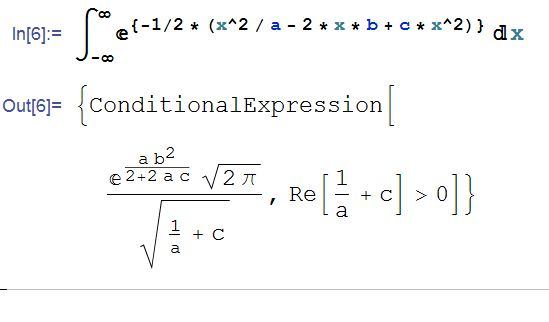
\includegraphics[width= 5.0in]{mathematica.jpg}
\end{figure}
\FloatBarrier

Plugging this result into the equation where the integral once was, we obtain:

\beqn
&=& \oneover{\tothepow{2\pi}{\overtwo{n} + 1}\sqrt{\sigsqmu \prod_{i=1}^{n} \sigsq_i}} \exp{-\half \sumonen{i}{\frac{R_i^2}{\sigsq_i}}} \sqrt{\frac{2\pi}{\oneover{\sigsq_\mu} + \displaystyle \sum_{i=1}^n \oneover{\sigsq_i}}} \exp{\frac{\sigsq_\mu \squared{\displaystyle \sum_{i=1}^n \frac{R_i}{\sigsq_i}}}{2 + 2\sigsq_\mu \displaystyle \sum_{i=1}^n \oneover{\sigsq_i}}}\\
&=& \oneover{\tothepow{2\pi}{\overtwo{n}}\sqrt{\parens{\displaystyle \prod_{i=1}^{n} \sigsq_i} \parens{1 + \sigsq_\mu \displaystyle \sum_{i=1}^n \oneover{\sigsq_i}}}} \exp{-\half \sumonen{i}{\frac{R_i^2}{\sigsq_i}}}  \exp{\overtwo{\sigsq_\mu} \parens{\frac{\squared{\displaystyle \sum_{i=1}^n \frac{R_i}{\sigsq_i}}}{1 + \sigsq_\mu \displaystyle \sum_{i=1}^n \oneover{\sigsq_i}}}}\\
\eeqn

Now we can solve for the likelihood ratio:

\beqn
\frac{\cprob{\R}{T^*, \sigsq_1, \ldots, \sigsq_n}}{\cprob{\R}{T, \sigsq_1, \ldots, \sigsq_n}} = \frac{\cprob{\R_L}{\sigsq_1, \ldots, \sigsq_n} \cprob{\R_R}{\sigsq}}{\cprob{\R}{\sigsq_1, \ldots, \sigsq_n}} \\
\eeqn

Note that there's many things that can cancel above. The sum of the $R_i^2 / \sigsq_i$'s would cancel numerator-denominator since we're adding the same set\footnote{The set of left leaf values $\cup$ the set of right leaf values has to equal the set of the node's parent's values}, the product of the $\sigsq_i$'s would cancel since we're multiplying over the same set, the $2\pi$'s will cancel as well leaving us with:

\begin{changemargin}{-20px}{0px}
\small
\beqn
&=& \sqrt{\frac{1 + \sigsq_\mu \displaystyle \sum_{i=1}^n \oneover{\sigsq_i}}{\parens{1 + \sigsq_\mu \displaystyle \sum_{i_L=1}^{n_L} \oneover{\sigsq_i}}\parens{1 + \sigsq_\mu \displaystyle \sum_{i_R=1}^{n_R} \oneover{\sigsq_i}}}}  \exp{\overtwo{\sigsq_\mu} \parens{\frac{\squared{\displaystyle \sum_{i_L=1}^{n_L} \frac{R_i}{\sigsq_i}}}{1 + \sigsq_\mu \displaystyle \sum_{i_L=1}^{n_L} \oneover{\sigsq_i}} + \frac{\squared{\displaystyle \sum_{i_R=1}^{n_R} \frac{R_i}{\sigsq_i}}}{1 + \sigsq_\mu \displaystyle \sum_{i_R=1}^{n_R} \oneover{\sigsq_i}} -  \frac{\squared{\displaystyle \sum_{i=1}^{n} \frac{R_i}{\sigsq_i}}}{1 + \sigsq_\mu \displaystyle \sum_{i=1}^{n} \oneover{\sigsq_i}}}}
\eeqn
\normalsize
\end{changemargin}

In log form this becomes:

\inblue{
\beqn
&& \half \parens{\natlog{1 + \sigsq_\mu \displaystyle \sum_{i=1}^{n} + \oneover{\sigsq_i}}} - \natlog{1 + \sigsq_\mu \displaystyle \sum_{i_L=1}^{n_L} \oneover{\sigsq_i}} - \natlog{1 + \sigsq_\mu \displaystyle \sum_{i_R=1}^{n_R} \oneover{\sigsq_i}} + \\
&& \overtwo{\sigsq_\mu} \parens{\frac{\squared{\displaystyle \sum_{i_L=1}^{n_L} \frac{R_i}{\sigsq_i}}}{1 + \sigsq_\mu \displaystyle \sum_{i_L=1}^{n_L} \oneover{\sigsq_i}} + \frac{\squared{\displaystyle \sum_{i_R=1}^{n_R} \frac{R_i}{\sigsq_i}}}{1 + \sigsq_\mu \displaystyle \sum_{i_R=1}^{n_R} \oneover{\sigsq_i}} -  \frac{\squared{\displaystyle \sum_{i=1}^{n} \frac{R_i}{\sigsq_i}}}{1 + \sigsq_\mu \displaystyle \sum_{i=1}^{n} \oneover{\sigsq_i}}}
\eeqn
}

\end{document}